%------------------------- Information ------------------------
% Compiler --> XeLaTeX because of the proprietary fonts
% In order to use the Eurostat chosen font "MyriadPro" you have to download theses fonts on https://fonts.adobe.com/fonts/myriad and save these file on the "FontsFiles" folder of your latex document
% alternatively, the use of Arial is permitted by Eurostat if Myriad Pro could not be use.

%------------------------- Parameters ------------------------

% Here you can choose the color theme of the document, see Eurostat Graphical style guide for details about wich one you have to choose : https://ec.europa.eu/eurostat/web/products-eurostat-news/-/STYLE-GUIDE_2016

%https://www.overleaf.com/project/5ec42a41ff549d0001f9ae37

% available options are : 
% - Theme1 : General and regional statistics
% - Theme2 : Economy and finance
% - Theme3 : Population and social conditions
% - Theme4 : Industry, trade and services
% - Theme5 : Agriculture and fisheries
% - Theme6 : International trade
% - Theme7 : Transport
% - Theme8 : Environment and energy
% - Theme9 : Science and technology

\documentclass[Theme1]{{template_material/eurostat}}

%------------------------- User packages ------------------------
% You can add packages here if you need any packages that is not already loaded by the eurostat class


%------------------------- Document variables ------------------------
% The 3 commands below have to be specified by user.
% They define variables that are displayed in different places in the document. 
% These locations are indicated in comments for each variable

\newcommand{\Articleedition}{2020 edition} % Cover, title
\newcommand{\Articleauthors}{Author One, Author Two, Author Three} % Cover, title
\newcommand{\Articletitle}{Eurostat {\LaTeX} Style Sheet} % Cover, title, footer

%------------------------- Document ------------------------
\begin{document}
%------------------------- Cover ------------------------
% cover
\thispagestyle{empty}
\pagenumbering{roman}
\begin{tikzpicture}[overlay,remember picture]
    
    % colored rectangle
    \fill[TH] (current page.north west) rectangle ++(\paperwidth,-80mm);
    
    % Title and authors
    \draw (current page.north west) ++ (138mm,-72mm) node[name=lefttextbox,above left,text width=118.5mm, align=right]{
            \fontsize{30pt}{33pt}\selectfont
            \textcolor{white}{\textbf{\Articletitle}} \\ \vspace{8mm}   
            \fontsize{14pt}{16pt}\selectfont 
            \textcolor{white}{\MakeUppercase{\textbf{\Articleauthors}}}
        };
    
    % Year
    \fontsize{24pt}{29pt}\selectfont
    \draw (current page.north west) ++ (148mm,-72mm) node[name=righttextbox,above right]{
        \textcolor{white}{\Articleedition}
        };
    
    % vertical ligne
    \draw (current page.north west) ++ (143mm,-85mm) node[name=bottomedot]{};
    \draw[white,very thick] (lefttextbox.north east)++(5mm,2mm) -- 
    (bottomedot);
    
    %---------------- editable graphical elements ----------------
    
    % cover picture
    \draw (current page.north) ++ (0mm,-79mm) node[name=cover_picture,below]{%
        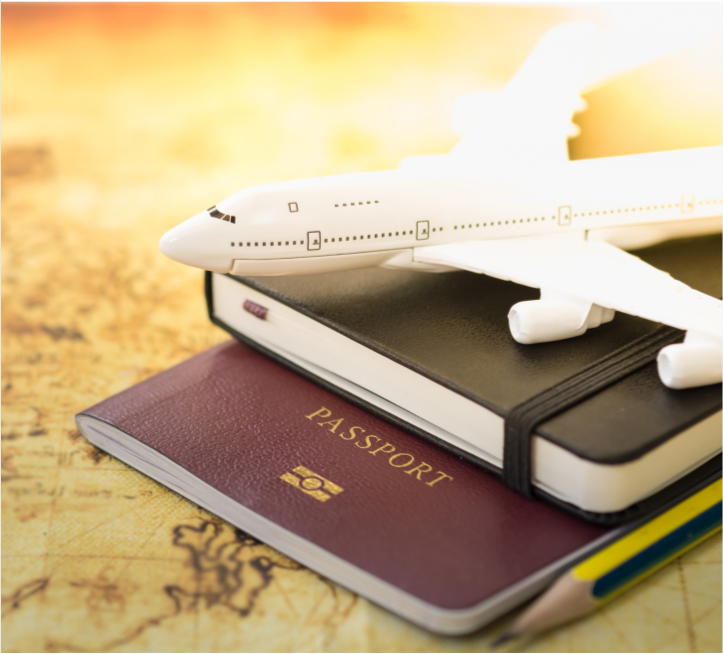
\includegraphics[width=21cm,height=19cm]{%
            template_material/PicturesFiles/coverpage_photo.PNG}
        };

    % co edition logo 1/1
    % \draw (current page.south west) ++ (38mm,12mm) node[name=coeditorlogo1,  right]{%
    %    
\includegraphics[height=23mm]{template_material/PicturesFiles/co-edition-logo-1.jpg}
    % }; 
     
    % co edition logo 1/2
    % \draw (current page.south west) ++ (1mm,12mm) node[name=coeditorlogoA,  right]{%
    %    
\includegraphics[height=23mm]{%
    %        template_material/PicturesFiles/co-edition-logo-1.jpg}
    %    }; 
     
    % co edition logo 2/2
    % \draw (current page.south west) ++ (25mm,12mm) node[name=coeditorlogoB,  right]{%
    %    
\includegraphics[height=18mm]{%
    %        template_material/PicturesFiles/co-edition-logo-2.png}
    %    }; 
     
    %---------------- end of the editable graphical elements ----------------
     
    % eurostat logo
     \draw (current page.south west) ++ (143mm,12mm) node[name=logo,  right]{
\includegraphics[width=65mm]{template_material/PicturesFiles/Logo_RGB-POS.png}};  
     
     % vertical ligne
    \draw (current page.south west) ++ (143mm,19mm) node[name=abovedotlogo]{};
    \draw (current page.south west) ++ (143mm,-5mm) node[name=botomedotlogo]{};
    \draw[gray65K,very thick] (abovedotlogo) -- (botomedotlogo);
    
    % collection
    \draw (current page.south west) ++ (138mm,9mm) node[name=lefttextbox,above left,text width=118.5mm, align=right]{
            \fontsize{10pt}{0pt}\selectfont
            \textcolor{gray65K}{STATISTICAL}
    };
    \draw (current page.south west) ++ (138mm,6.3mm) node[name=lefttextbox,above left,text width=118.5mm, align=right]{
        \fontsize{10pt}{0pt}\selectfont
        \textcolor{gray65K}{PAPERS}
    };
    \draw (current page.south west) ++ (126mm,6.3mm) node[name=lefttextbox,above left,text width=118.5mm, align=right]{
        \fontsize{10pt}{0pt}\selectfont
        \textcolor{gray65K}{WORKING}
    };
\end{tikzpicture}
\restoregeometry
% blank page
\newpage \thispagestyle{empty} \mbox{} 
%------------------------- Title page ------------------------
% title page
\newpage 
\thispagestyle{empty}
\pagenumbering{arabic}
\begin{tikzpicture}[overlay,remember picture]
    
    % Title and authors
    \draw (current page.north west) ++ (138mm,-72mm) node[name=lefttextbox,above left,text width=118.5mm, align=right]{
            \fontsize{30pt}{33pt}\selectfont
            \textcolor{gray65K}{\Articletitle} \\ \vspace{8mm}   
            \fontsize{14pt}{16pt}\selectfont 
            \textcolor{gray65K}{\MakeUppercase{\textbf{\Articleauthors}}}
        };
    
    % Year
    \fontsize{24pt}{29pt}\selectfont
    \draw (current page.north west) ++ (148mm,-72mm) node[name=righttextbox,above right]{
        \textcolor{gray65K}{\Articleedition}
        };
    
    % vertical ligne
    \draw (current page.north west) ++ (143mm,-85mm) node[name=bottomedot]{};
    \draw[gray65K,very thick] (lefttextbox.north east)++(5mm,4mm) -- 
    (bottomedot);
    
\end{tikzpicture}
\restoregeometry
%------------------------- Copyright page ------------------------
\newpage
\thispagestyle{empty}
\newgeometry{left=2cm,right=3cm,bottom=4cm}

\vspace*{\fill}


\textit{Printed by [Xxx] in [Country]}

Manuscript completed in [Month] [Year]

[Revised/Corrected/nth] edition {\color{red}[if needed]}

The European Commission is not liable for any consequence stemming from the reuse of this publication. 

Luxembourg: Publications Office of the European Union, [Year]

© European Union, [Year] 


\includegraphics[width=3cm]{template_material/PicturesFiles/creative_commons_by.png}

The reuse policy of European Commission documents is implemented based on Commission Decision 2011/833/EU of 12 December 2011 on the reuse of Commission documents (OJ L 330, 14.12.2011, p. 39).
Except otherwise noted, the reuse of this document is authorised under a Creative Commons Attribution 4.0 International (CC-BY 4.0) licence (https://creativecommons.org/licenses/by/4.0/). This means that reuse is allowed provided appropriate credit is given and any changes are indicated.
For any use or reproduction of elements that are not owned by the European Union, permission may need to be sought directly from the respective rightholders. 

{\color{red}[or]}

For any use or reproduction of elements that are not owned by the European Union, permission may need to be sought directly from the respective rightholders. The European Union does not own the copyright in relation to the following elements:
[cover], [element concerned], [source: e.g. Fotolia.com];
[page XX], [element by XX] [source: e.g. Unsplash.com].

Theme:\\
Collection: 

Print	ISBN xxx-xx-xx-xxxxx-x	ISSN xxxx-xxxx	doi:10.xxxx/xx...x	xx-xx-xx-xxx-xx-x
PDF	ISBN xxx-xx-xx-xxxxx-x	ISSN xxxx-xxxx	doi:10.xxxx/xx...x	xx-xx-xx-xxx-xx-x

\begin{tabbing}
Print \hspace{1cm}\= ISBN xxx-xx-xx-xxxxx-x \hspace{1cm}\= ISSN xxxx-xxxx \hspace{1cm}\= doi:10.xxxx/xx...x \hspace{1cm}\= xx-xx-xx-xxx-xx-x\\
PDF	\> ISBN xxx-xx-xx-xxxxx-x \> ISSN xxxx-xxxx \> doi:10.xxxx/xx...x \> xx-xx-xx-xxx-xx-x
\end{tabbing}

\restoregeometry
%------------------------- Pagestyle ------------------------
%Keep this before the first section of your article and after the copryght page.
% header
\pagestyle{numstyle} % required for footer and header
\renewcommand{\sectionmark}[1]{\markboth{#1}{}} % define /sectionmark to avoid showing the section number in the header.
%------------------------- Abstract ------------------------
\newpage
\addcontentsline{toc}{section}{Abstract} % Add the abstract section to the table of contents
\section*{Abstract}

\lipsum[1-2] % Dummy text

\textbf{Keywords: } Keyword one, Keyword two, Keyword three, Keyword four.

\textbf{Authors: } Author one \footnote{footnote information about author one : affiliation, author.one@email.com}, Author two \footnote{footnote information about author two : affiliation, author.two@email.com}, Author three \footnote{footnote information about author three : affiliation,  author.three@email.com}.

\textbf{Acknowledgement: } \lipsum[1-1]


\newpage % If the /newpage command is not present before each section, the header could show the wrong section number and title.

%------------------------- Table of content ------------------------
\begingroup
\renewcommand*\contentsname{Table of contents}
\setlength{\parskip}{4pt}
\renewcommand{\cftsecfont}{\bfseries\fontsize{11pt}{8pt}\selectfont}
\renewcommand{\cftsubsecfont}{\bfseries}

\renewcommand{\cftdotsep}{0.5}
\renewcommand{\cftsecleader}{\bfseries\fontsize{11pt}{8pt}\cftdotfill{\cftdotsep}}
\renewcommand{\cftsubsecleader}{\bfseries\cftdotfill{\cftdotsep}}

%\addcontentsline{toc}{section}{Table of contents} % Add the section to the table of contents
\tableofcontents

\endgroup
\newpage % If the /newpage command is not present before each section, the header could show the wrong section number and title. 


%------------------------- Body ------------------------

\section{How to use this template}

This template provides examples for the basic functionalities needed in article writing. The examples provided in the next sections can be copied and modified as needed.

\subsection{About eurostat class}

The eurostat class is a custom class created to help Eurostat researchers to easily edit their articles with LaTeX and follow Eurostat graphical guidelines. 

\subsubsection{Packages used by Eurostat class}

The eurostat class is based on the article class. The list of the packages used by eurostat class is as follow:
\begin{minted}{latex}
\RequirePackage[a4paper]{geometry}
\RequirePackage[table,xcdraw]{xcolor}
\RequirePackage[explicit]{titlesec} % Required for the titles formating
\RequirePackage{fancyhdr} % require for header and footer
\RequirePackage{marvosym} % required for the symbols 
\RequirePackage{xparse} % required for unnumbered section names in header
\RequirePackage{graphicx} % Required for including pictures
\RequirePackage{caption} % Required for caption format
\RequirePackage{subcaption} % Required for caption in multi plots
\RequirePackage[hang,flushmargin]{footmisc} % Required for footnotes (kill the indentation)
\RequirePackage{pdflscape} % Required for landscape pages
\RequirePackage{multirow} % Required for tables
\RequirePackage{fontspec} %fonts
\RequirePackage{minted} %display code chunk
\RequirePackage{lipsum}% just to generate text for the example
\RequirePackage{tikz} % Required to draw 
\RequirePackage[many]{tcolorbox} % Required for boxes
\RequirePackage[titles]{tocloft} % Required for the table of contents
\RequirePackage{natbib} % Required for quotes style
\RequirePackage{multicol,multirow}
\RequirePackage{amsmath,amssymb,amsfonts}
\RequirePackage{mathrsfs}
\RequirePackage{amsthm}
\RequirePackage{rotating}
\RequirePackage{appendix}
\end{minted}

If you want to use any other packages, you can add them in the preamble of the main.tex file. 

\newpage
\subsubsection{XeLatex}

The eurostat class will only work with Xelatex. Due to the font used, Myriad Pro, we have to use the fontspec package which only works with Xelatex and lualatex. Eurostat class may work with lualatex but it is not tested. 

\subsection{Choosing the theme}

Eurostat statistics cover a wide range of topics. These topics are organised in nine different themes reflecting a statistical category. Each publication refers to one of these themes shown in Figure 1. 

\begin{figure}[h]
    % figure centering result on a non aligned caption, the caption will stay aligned with the right side of the page. 
    \caption{List of themes} % caption have to appear above the figure
    \label{fig:listofthemes}
    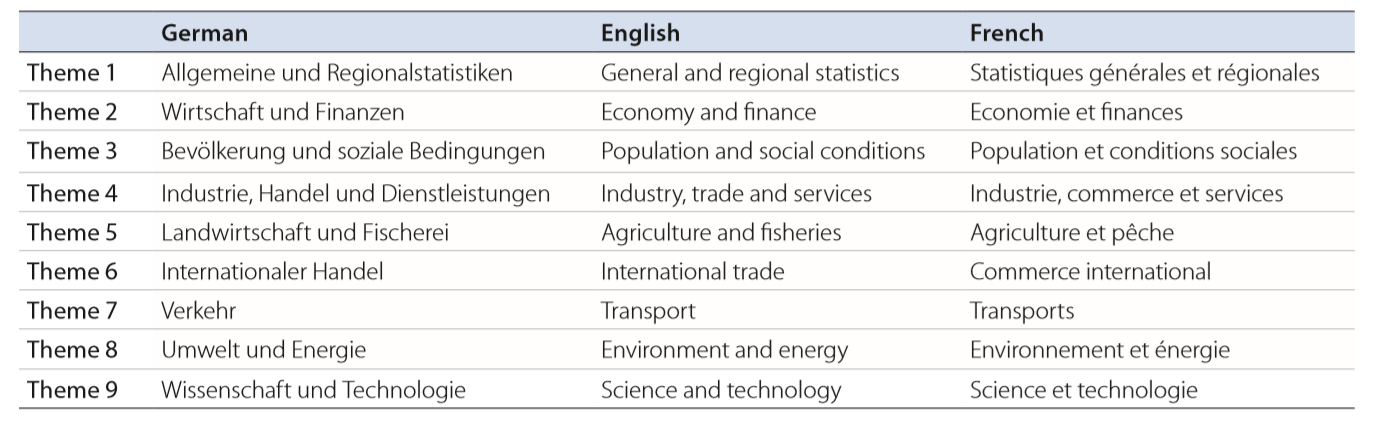
\includegraphics[width=1\textwidth]{template_material/FiguresFiles/List of themes.PNG}
\end{figure}

Each Eurostat theme is distinguished by a different colour.  The colours chosen for the themes are all medium tones, so that black text as well as white text, when used with these colours, remains readable.
The use of these colours on the cover pages, in the layout and for data visualisation strongly contributes to the identification of Eurostat’s publications. They are founding elements of the graphical charter (Figure 2 and Figure 3).

\begin{figure}[h]
    % figure centering result on a non aligned caption, the caption will stay aligned with the right side of the page. 
    \caption{Theme colours} % caption have to appear above the figure
    \label{fig:themecolours}
    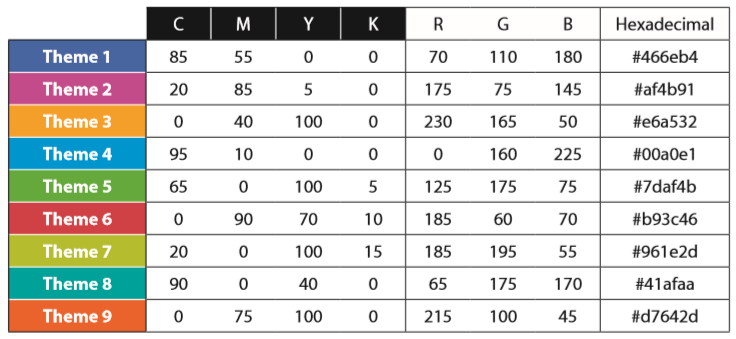
\includegraphics[width=1\textwidth]{template_material/FiguresFiles/Theme_colours.PNG}
\end{figure}

\begin{figure}[h]
    % figure centering result on a non aligned caption, the caption will stay aligned with the right side of the page. 
    \caption{Colours palette} % caption have to appear above the figure
    \label{fig:themecolourspalette}
    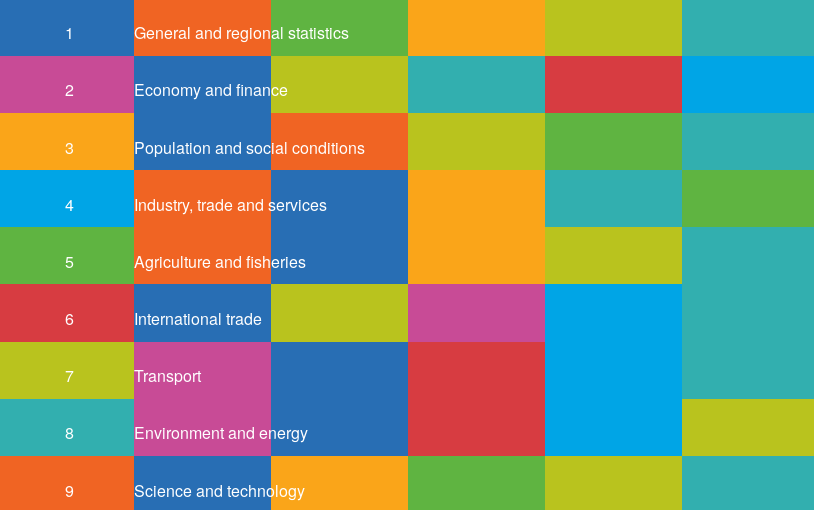
\includegraphics[width=1\textwidth]{template_material/FiguresFiles/themes_colours_palette.png}
\end{figure}

\newpage
The colors of this template can be modified to correspond to one of the 9 themes with a simple modification. To select the topic corresponding to your article, please find the command \cs{documentclass[]\{\}} at the beginning of the main.tex file. Then you need to change the option. Available options are:

\begin{table}[h]
    \caption{Class eurostat options\label{tab_class_options}}
    \begin{tabular}{l|l}
    \hlinesep
    \rowcolor{TH20p}
    \multicolumn{1}{c}{\bf Option} & \multicolumn{1}{c}{\bf Topic}   \\ \hlinesep
    Theme1    & General and regional statistics   \\
    Theme2    & Economy and finance   \\
    Theme3    & Population and social conditions   \\
    Theme4    & Industry, trade and services   \\
    Theme5    & Agriculture and fisheries   \\
    Theme6    & International trade   \\
    Theme7    & Transport   \\
    Theme8    & Environment and energy   \\
    Theme9    & Science and technology   \\ \hlinesep
    \end{tabular}
\end{table}

For instance, if you want to use Theme 8, the  \cs{documentclass[]\{\}} command should be : 

\begin{minted}{latex}
\documentclass[Theme8]{{template_material/eurostat}}
\end{minted}

\subsection{Editing cover image and co-editions logo}

To edit any of the graphical elements of the cover, go to the cover.tex file in the template\_material folder. You will find a section delimited by a comment called "editable graphical elements". 

The graphicals elements are defined by \cs{includegraphics[]\{\}} commands. Each of the \cs{includegraphics[]\{\}} commands are included in a \cs{draw} command. 

\begin{minted}{latex}
%---------------- editable graphical elements ----------------
    
% cover picture
\draw (current page.north) ++ (0mm,-79mm) node[name=cover_picture,below]{%
    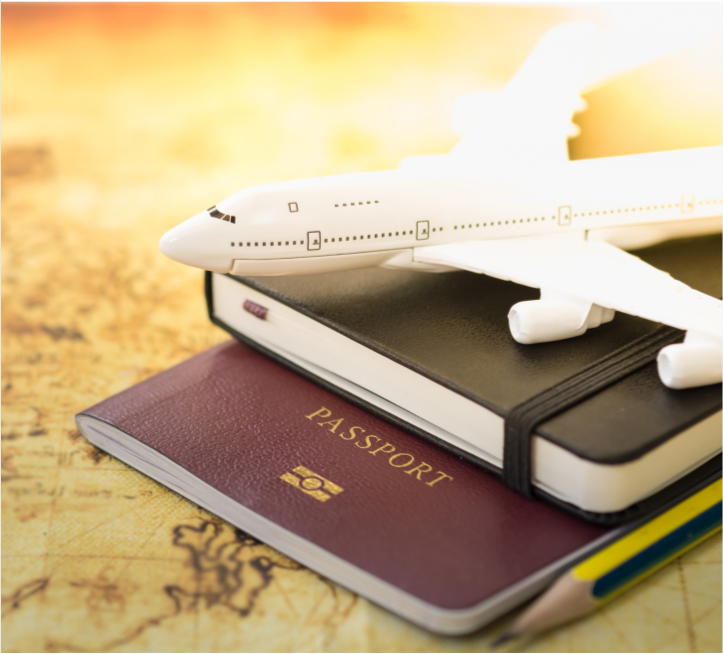
\includegraphics[width=21cm,height=19cm]{%
        template_material/PicturesFiles/coverpage_photo.PNG}
    };

% co edition logo 1/1
% \draw (current page.south west) ++ (38mm,12mm) node[name=coeditorlogo1,  right]{%
%    
\includegraphics[height=23mm]{template_material/PicturesFiles/co-edition-logo-1.jpg}
% }; 
     
% co edition logo 1/2
 \draw (current page.south west) ++ (10mm,12mm) node[name=coeditorlogoA,  right]{%
    
\includegraphics[height=23mm]{%
        template_material/PicturesFiles/co-edition-logo-1.jpg}
    }; 
     
% co edition logo 2/2
 \draw (current page.south west) ++ (65mm,12mm) node[name=coeditorlogoB,  right]{%
    
\includegraphics[height=18mm]{%
        template_material/PicturesFiles/co-edition-logo-2.png}
    }; 
%---------------- end of the editable graphical elements ----------------
\end{minted}

Also, you can easily create your own cover page by copying and editing the cover.tex file. After renaming your copy, and can put it in another folder, to include it in your article, go to the main.tex file, find and edit the following command to adjust the path of the cover file :
\begin{minted}{latex}
\thispagestyle{empty}
\pagenumbering{roman}
\begin{tikzpicture}[overlay,remember picture]
    
    % colored rectangle
    \fill[TH] (current page.north west) rectangle ++(\paperwidth,-80mm);
    
    % Title and authors
    \draw (current page.north west) ++ (138mm,-72mm) node[name=lefttextbox,above left,text width=118.5mm, align=right]{
            \fontsize{30pt}{33pt}\selectfont
            \textcolor{white}{\textbf{\Articletitle}} \\ \vspace{8mm}   
            \fontsize{14pt}{16pt}\selectfont 
            \textcolor{white}{\MakeUppercase{\textbf{\Articleauthors}}}
        };
    
    % Year
    \fontsize{24pt}{29pt}\selectfont
    \draw (current page.north west) ++ (148mm,-72mm) node[name=righttextbox,above right]{
        \textcolor{white}{\Articleedition}
        };
    
    % vertical ligne
    \draw (current page.north west) ++ (143mm,-85mm) node[name=bottomedot]{};
    \draw[white,very thick] (lefttextbox.north east)++(5mm,2mm) -- 
    (bottomedot);
    
    %---------------- editable graphical elements ----------------
    
    % cover picture
    \draw (current page.north) ++ (0mm,-79mm) node[name=cover_picture,below]{%
        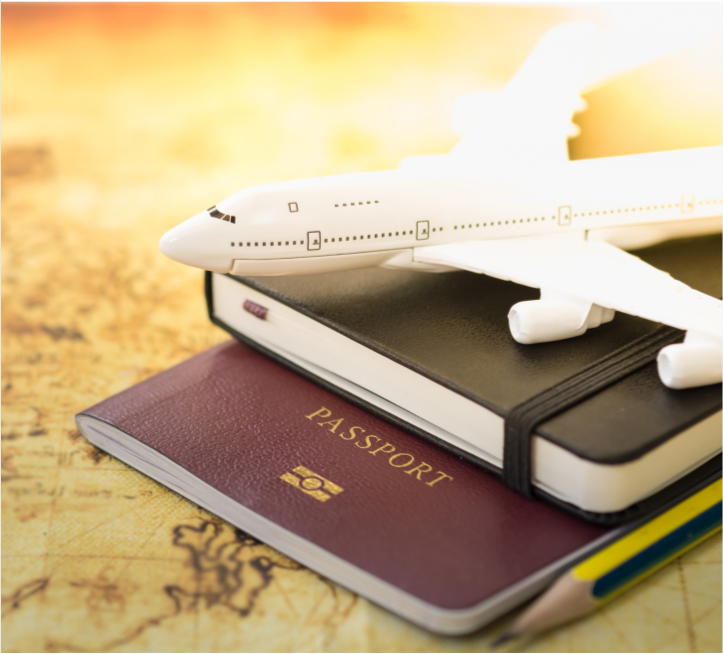
\includegraphics[width=21cm,height=19cm]{%
            template_material/PicturesFiles/coverpage_photo.PNG}
        };

    % co edition logo 1/1
    % \draw (current page.south west) ++ (38mm,12mm) node[name=coeditorlogo1,  right]{%
    %    
\includegraphics[height=23mm]{template_material/PicturesFiles/co-edition-logo-1.jpg}
    % }; 
     
    % co edition logo 1/2
    % \draw (current page.south west) ++ (1mm,12mm) node[name=coeditorlogoA,  right]{%
    %    
\includegraphics[height=23mm]{%
    %        template_material/PicturesFiles/co-edition-logo-1.jpg}
    %    }; 
     
    % co edition logo 2/2
    % \draw (current page.south west) ++ (25mm,12mm) node[name=coeditorlogoB,  right]{%
    %    
\includegraphics[height=18mm]{%
    %        template_material/PicturesFiles/co-edition-logo-2.png}
    %    }; 
     
    %---------------- end of the editable graphical elements ----------------
     
    % eurostat logo
     \draw (current page.south west) ++ (143mm,12mm) node[name=logo,  right]{
\includegraphics[width=65mm]{template_material/PicturesFiles/Logo_RGB-POS.png}};  
     
     % vertical ligne
    \draw (current page.south west) ++ (143mm,19mm) node[name=abovedotlogo]{};
    \draw (current page.south west) ++ (143mm,-5mm) node[name=botomedotlogo]{};
    \draw[gray65K,very thick] (abovedotlogo) -- (botomedotlogo);
    
    % collection
    \draw (current page.south west) ++ (138mm,9mm) node[name=lefttextbox,above left,text width=118.5mm, align=right]{
            \fontsize{10pt}{0pt}\selectfont
            \textcolor{gray65K}{STATISTICAL}
    };
    \draw (current page.south west) ++ (138mm,6.3mm) node[name=lefttextbox,above left,text width=118.5mm, align=right]{
        \fontsize{10pt}{0pt}\selectfont
        \textcolor{gray65K}{PAPERS}
    };
    \draw (current page.south west) ++ (126mm,6.3mm) node[name=lefttextbox,above left,text width=118.5mm, align=right]{
        \fontsize{10pt}{0pt}\selectfont
        \textcolor{gray65K}{WORKING}
    };
\end{tikzpicture}
\restoregeometry
\end{minted}

\subsubsection{Cover picture}

To edit the cover picture, find the \cs{includegraphics[]\{\}} commands below the comment "\% cover picture", then edit the picture path as desired.

To be displayed correctly, the picture must be 210 mm width and 190 mm heigth. 

\subsubsection{co-editors logo}

You can choose between the following three situations:
\begin{enumerate}
    \item There is no co-editor
    \item There is one co-editor
    \item There is two co-editors
\end{enumerate}


\newpage
\paragraph{No co-editor}

In the first case, no co-editor, you must edit the cover.tex file to comment all of the co-editors logo pictures as in the following example:

\begin{minted}{latex}
%---------------- editable graphical elements ----------------
    
% cover picture
\draw (current page.north) ++ (0mm,-79mm) node[name=cover_picture,below]{%
    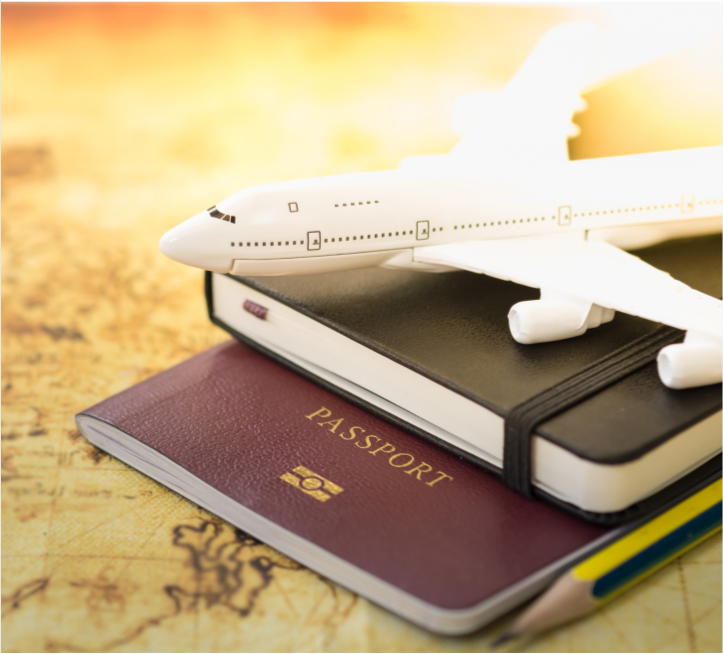
\includegraphics[width=21cm,height=19cm]{%
        template_material/PicturesFiles/coverpage_photo.PNG}
    };

% co edition logo 1/1
% \draw (current page.south west) ++ (38mm,12mm) node[name=coeditorlogo1,  right]{%
%    
\includegraphics[height=23mm]{template_material/PicturesFiles/co-edition-logo-1.jpg}
% }; 
     
% co edition logo 1/2
% \draw (current page.south west) ++ (10mm,12mm) node[name=coeditorlogoA,  right]{%
%    
\includegraphics[height=23mm]{%
%        template_material/PicturesFiles/co-edition-logo-1.jpg}
%    }; 
     
% co edition logo 2/2
% \draw (current page.south west) ++ (65mm,12mm) node[name=coeditorlogoB,  right]{%
%    
\includegraphics[height=18mm]{%
%        template_material/PicturesFiles/co-edition-logo-2.png}
%    }; 

%---------------- end of the editable graphical elements ----------------
\end{minted}

\paragraph{One co-editor}

In the second case, only one co-editor, you must edit the cover.tex file to comment the co-editors logo pictures 1/2 and 2/2 as in the following example. Then, you must edit the co-editor logo path in the \cs{includegraphics[]\{\}} command.
\begin{minted}{latex}
%---------------- editable graphical elements ----------------
    
% cover picture
\draw (current page.north) ++ (0mm,-79mm) node[name=cover_picture,below]{%
    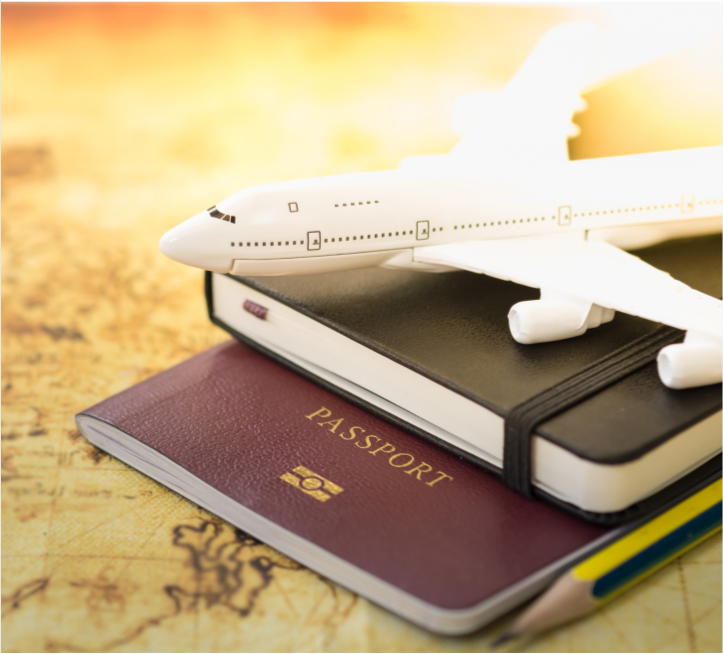
\includegraphics[width=21cm,height=19cm]{%
        template_material/PicturesFiles/coverpage_photo.PNG}
    };

% co edition logo 1/1
 \draw (current page.south west) ++ (38mm,12mm) node[name=coeditorlogo1,  right]{%
    
\includegraphics[height=23mm]{template_material/PicturesFiles/co-edition-logo-1.jpg}
 }; 
     
% co edition logo 1/2
% \draw (current page.south west) ++ (10mm,12mm) node[name=coeditorlogoA,  right]{%
%    
\includegraphics[height=23mm]{%
%        template_material/PicturesFiles/co-edition-logo-1.jpg}
%    }; 
     
% co edition logo 2/2
% \draw (current page.south west) ++ (65mm,12mm) node[name=coeditorlogoB,  right]{%
%    
\includegraphics[height=18mm]{%
%        template_material/PicturesFiles/co-edition-logo-2.png}
%    }; 

%---------------- end of the editable graphical elements ----------------
\end{minted}

\paragraph{Two co-editors}

In the third case, two co-editors, you must edit the cover.tex file to comment the co-editor logo pictures 1/1 as in the following example. Then, you must edit the co-editors logo paths in the \cs{includegraphics[]\{\}} commands.
\begin{minted}{latex}
%---------------- editable graphical elements ----------------
% cover picture
\draw (current page.north) ++ (0mm,-79mm) node[name=cover_picture,below]{%
    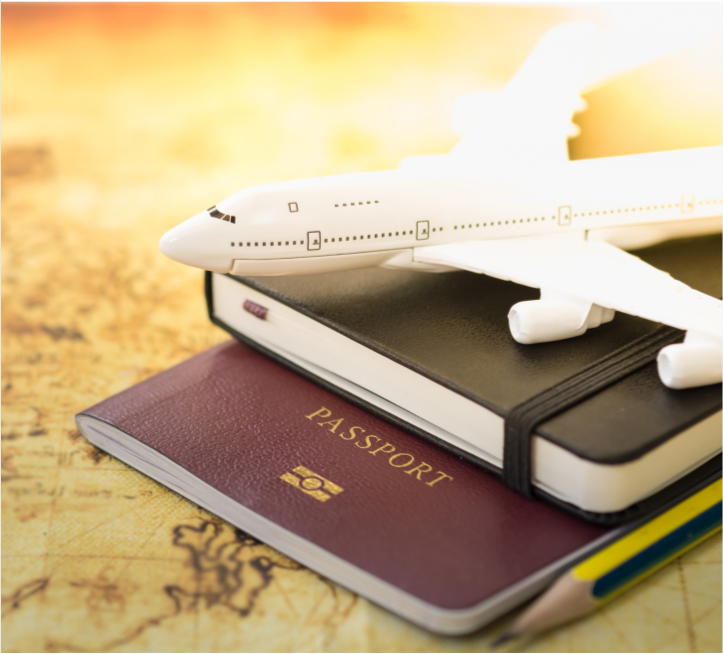
\includegraphics[width=21cm,height=19cm]{%
        template_material/PicturesFiles/coverpage_photo.PNG}
    };

% co edition logo 1/1
% \draw (current page.south west) ++ (38mm,12mm) node[name=coeditorlogo1,  right]{%
%    
\includegraphics[height=23mm]{template_material/PicturesFiles/co-edition-logo-1.jpg}
% }; 
     
% co edition logo 1/2
 \draw (current page.south west) ++ (10mm,12mm) node[name=coeditorlogoA,  right]{%
    
\includegraphics[height=23mm]{%
        template_material/PicturesFiles/co-edition-logo-1.jpg}
    }; 
     
% co edition logo 2/2
 \draw (current page.south west) ++ (65mm,12mm) node[name=coeditorlogoB,  right]{%
    
\includegraphics[height=18mm]{%
        template_material/PicturesFiles/co-edition-logo-2.png}
    }; 

%---------------- end of the editable graphical elements ----------------
\end{minted}

\paragraph{Adjusting logo size}

The displayed size of the co-editors logo could be adjusted using the height option of the \cs{includegraphics[]\{\}} command.

\newpage
\subsection{Defining the title, the year and the authors list}

In the preamble of the main.tex file you will find a section called "document variables". Here you can edit the year, the title and the authors list of you article. 

\begin{minted}{latex}
%------------------------- Document variables ------------------------
% The 3 commands below have to be specified by user.
% They define variables that are displayed in different places in the document. 
% These locations are indicated in comments for each variable

\newcommand{\Articleedition}{2019 edition} % Cover, title
\newcommand{\Articleauthors}{Author One, Author Two, Author Three} % Cover, title
\newcommand{\Articletitle}{Eurostat Style Sheet} % Cover, title, footer
\end{minted}

\subsection{The copyright page}

Like the cover page, the copyright page is defined by a separate .tex file. You can find it in the template\_material folder and include it in the main.tex file with the following command. 
\begin{minted}{latex}
\thispagestyle{empty}
\newgeometry{left=2cm,right=3cm,bottom=4cm}

\vspace*{\fill}


\textit{Printed by [Xxx] in [Country]}

Manuscript completed in [Month] [Year]

[Revised/Corrected/nth] edition {\color{red}[if needed]}

The European Commission is not liable for any consequence stemming from the reuse of this publication. 

Luxembourg: Publications Office of the European Union, [Year]

© European Union, [Year] 


\includegraphics[width=3cm]{template_material/PicturesFiles/creative_commons_by.png}

The reuse policy of European Commission documents is implemented based on Commission Decision 2011/833/EU of 12 December 2011 on the reuse of Commission documents (OJ L 330, 14.12.2011, p. 39).
Except otherwise noted, the reuse of this document is authorised under a Creative Commons Attribution 4.0 International (CC-BY 4.0) licence (https://creativecommons.org/licenses/by/4.0/). This means that reuse is allowed provided appropriate credit is given and any changes are indicated.
For any use or reproduction of elements that are not owned by the European Union, permission may need to be sought directly from the respective rightholders. 

{\color{red}[or]}

For any use or reproduction of elements that are not owned by the European Union, permission may need to be sought directly from the respective rightholders. The European Union does not own the copyright in relation to the following elements:
[cover], [element concerned], [source: e.g. Fotolia.com];
[page XX], [element by XX] [source: e.g. Unsplash.com].

Theme:\\
Collection: 

Print	ISBN xxx-xx-xx-xxxxx-x	ISSN xxxx-xxxx	doi:10.xxxx/xx...x	xx-xx-xx-xxx-xx-x
PDF	ISBN xxx-xx-xx-xxxxx-x	ISSN xxxx-xxxx	doi:10.xxxx/xx...x	xx-xx-xx-xxx-xx-x

\begin{tabbing}
Print \hspace{1cm}\= ISBN xxx-xx-xx-xxxxx-x \hspace{1cm}\= ISSN xxxx-xxxx \hspace{1cm}\= doi:10.xxxx/xx...x \hspace{1cm}\= xx-xx-xx-xxx-xx-x\\
PDF	\> ISBN xxx-xx-xx-xxxxx-x \> ISSN xxxx-xxxx \> doi:10.xxxx/xx...x \> xx-xx-xx-xxx-xx-x
\end{tabbing}

\restoregeometry
\end{minted}

You can copy and edit your own version of the copyright page, and edit the path in the corresponding \cs{include\{\}} command in the main.tex file. 


\subsection{Numbered and unnumbered sections}

The unnumbered sections should not be used after the first numbered section and before the last numbered section. The Header show the name and the number of the section. If an unnumbered section is used the header will not display the section number. The other unnumbered levels can be used anywhere in the document.

\begin{boxe3}{Section numbering in headers}
    It is necessary to use the \cs{newpage} commande before the \cs{section\{\}} command. If the \cs{newpage} command is missing, you will notice section numbering errors in the headers.
\end{boxe3}

\subsection{The template material folder}

The template\_material folder contains all the necessary files to use the style sheet and should not be edited. 

You can copy the elements that you need to modify and then change the paths to these elements in the main.tex file.

The main\_copy.tex file is a backup of the main.tex file. If you change something by accident in the process of writing your article, you can use the main\_copy.tex file to fix it. 

\newpage % If the /newpage command is not present before each section, the header could show the wrong section number and title. 
\section{Numbered sections and subsections titles}
Lorem ipsum dolor sit amet, consectetuer adipiscing elit. Ut purus elit, vestibulum ut, placerat ac, adip-iscing vitae, felis. Curabitur dictum gravida mauris. Nam arcu libero, nonummy eget, consectetuer id,vulputate a, magna. Donec vehicula augue eu neque.
\subsection{H1 Sub section title}
Lorem ipsum dolor sit amet, consectetuer adipiscing elit. Ut purus elit, vestibulum ut, placerat ac, adip-iscing vitae, felis. Curabitur dictum gravida mauris. Nam arcu libero, nonummy eget, consectetuer id,vulputate a, magna. Donec vehicula augue eu neque.
\subsubsection{H2 Sub sub section title}
Lorem ipsum dolor sit amet, consectetuer adipiscing elit. Ut purus elit, vestibulum ut, placerat ac, adip-iscing vitae, felis. Curabitur dictum gravida mauris. Nam arcu libero, nonummy eget, consectetuer id,vulputate a, magna. Donec vehicula augue eu neque.
\paragraph{H3 Paragraph title}
Lorem ipsum dolor sit amet, consectetuer adipiscing elit. Ut purus elit, vestibulum ut, placerat ac, adip-iscing vitae, felis. Curabitur dictum gravida mauris. Nam arcu libero, nonummy eget, consectetuer id,vulputate a, magna. Donec vehicula augue eu neque.
\subparagraph{H4 Sub paragraph title}
Lorem ipsum dolor sit amet, consectetuer adipiscing elit. Ut purus elit, vestibulum ut, placerat ac, adip-iscing vitae, felis. Curabitur dictum gravida mauris. Nam arcu libero, nonummy eget, consectetuer id,vulputate a, magna. Donec vehicula augue eu neque.
\newpage % If the /newpage command is not present before each section, the header could show the wrong section number and title. 

\section*{H1 Unnumbered sections and subsections titles}

The unnumbered section should not be used after the first numbered section and before the last numbered section. The Header show the name and the number of the section. If an unnumbered section is used the header will not show the number. 

\subsection*{H2 Sub section title unnumbered }

The other levels could be use anywhere in the document.

\subsubsection*{H3 Sub sub section title unnumbered}

Lorem ipsum dolor sit amet, consectetuer adipiscing elit. Ut purus elit, vestibulum ut, placerat ac, adip-iscing vitae, felis. Curabitur dictum gravida mauris. Nam arcu libero, nonummy eget, consectetuer id,vulputate a, magna. Donec vehicula augue eu neque.

\paragraph*{H4 Paragraph title unnumbered}
Lorem ipsum dolor sit amet, consectetuer adipiscing elit. Ut purus elit, vestibulum ut, placerat ac, adip-iscing vitae, felis. Curabitur dictum gravida mauris. Nam arcu libero, nonummy eget, consectetuer id,vulputate a, magna. Donec vehicula augue eu neque.

\subparagraph*{H5 Sub paragraph title unnumbered}
Lorem ipsum dolor sit amet, consectetuer adipiscing elit. Ut purus elit, vestibulum ut, placerat ac, adip-iscing vitae, felis. Curabitur dictum gravida mauris. Nam arcu libero, nonummy eget, consectetuer id,vulputate a, magna. Donec vehicula augue eu neque.

\subsubparagraph{H6 Sub sub paragraph title unnumbered} 
Lorem ipsum dolor sit amet, consectetuer adipiscing elit. Ut purus elit, vestibulum ut, placerat ac, adip-iscing vitae, felis. Curabitur dictum gravida mauris. Nam arcu libero, nonummy eget, consectetuer id,vulputate a, magna. Donec vehicula augue eu neque.

\newpage % If the /newpage command is not present before each section, the header could show the wrong section number and title. 

\section{Section and subsection title with lorem}



\subsection{H1 Sub section title H1}
\lipsum[1-1]
\subsubsection{H2 The sub sub section title H2}
\lipsum[1-1]
\paragraph{H3 The sub sub sub section title H3}
\lipsum[1-1]
\subparagraph{H4 sub paragraph H4}
\lipsum[1-1]

\newpage % If the /newpage command is not present before each section, the header could show the wrong section number and title. 
\section{Unordered lists and ordered lists}

\subsection{Unordered lists}
 \begin{itemize}
   \item  First Level
   \begin{itemize}
     \item  Second Level
     \begin{itemize}
       \item  Third Level
       \begin{itemize}
         \item  Fourth Level
       \end{itemize}
     \end{itemize}
   \end{itemize}
 \end{itemize}

\subsection{Ordered lists}
\begin{enumerate}
   \item First level item
   \item First level item
   \begin{enumerate}
     \item Second level item
     \item Second level item
     \begin{enumerate}
       \item Third level item
       \item Third level item
       \begin{enumerate}
         \item Fourth level item
         \item Fourth level item
       \end{enumerate}
     \end{enumerate}
   \end{enumerate}
 \end{enumerate}
\newpage % If the /newpage command is not present before each section, the header could show the wrong section number and title. 


\section{Hyperlinks}

Here is an hyperlink to Eurostat main page : \href{https://ec.europa.eu/eurostat/fr/home}{Eurostat} 

Here is an example for a simple url display : \url{https://ec.europa.eu/eurostat/fr/home}

\newpage % If the /newpage command is not present before each section, the header could show the wrong section number and title. 


\section{Boxes}

\begin{boxe1}{Box title}
    This is the text formatted by the boxed environment
    \begin{itemize}
        \item Body bullet list
    \end{itemize}
\end{boxe1}

\vspace{1cm}

\begin{boxe2}{Box title}
    Body text \\
    \boldthcolor{Body theme colour bold (you can also put some coloured text inside)} \\
    Background = theme colour 20
\end{boxe2}

\vspace{1cm}

\begin{boxe3}{Box title white}
    Body white bold \\
    Background = theme colour \\
    This kind of box should be avoided for content with more than 15 lines
\end{boxe3}

\newpage % If the /newpage command is not present before each section, the header could show the wrong section number and title. 
\section{Figures}

\subsection{Left aligned figure}

Here is an example for inserting a figure with caption and reference :
You can cite your figure in your text like this : figure \ref{fig:figure1}

Please be carefull to keep the \cs{caption\{\}} command at the begening of the figure environment. Accordind to the Eurostat graphical guidelines, the caption have to be always placed above the figure.

\begin{figure}[h]
    % figure centering result on a non aligned caption, the caption will stay aligned with the right side of the page. 
    \caption{a nice plot} % caption have to appear above the figure
    \label{fig:figure1}
    
\includegraphics[width=0.6\textwidth]{template_material/FiguresFiles/Simple_supply_and_demand.svg.png}
\end{figure}

\newpage
\subsection{Centered figure}

Here is an exemple of a centered figure. You have to use the \cs{centering} command just before the \cs{includegraphics} command. As you can see, the caption is always aligned left with the left margin even if the figure is centered. 

Please be carefull to keep the \cs{caption\{\}} command at the begening of the figure environment. Accordind to the Eurostat graphical guidelines, the caption have to be always placed above the figure.

\begin{figure}[h]
    % figure centering result on a non aligned caption, the caption will stay aligned with the right side of the page. 
    \caption{a centered figure} % caption have to appear above the figure
    \label{fig:figure2}
    \centering
    
\includegraphics[width=0.7\textwidth]{template_material/FiguresFiles/Simple_supply_and_demand.svg.png}
\end{figure}

\newpage
\subsection{Subfigures}

Here is an exemple of how to insert subfigures. 

Please be carefull to keep the \cs{caption\{\}} command at the begening of the figure environment. Accordind to the Eurostat graphical guidelines, the caption have to be always placed above the figure.

\begin{figure}[h]
    \caption{Three simple graphs}
    \label{fig:three graphs}
     \centering
     \begin{subfigure}[b]{0.3\textwidth}
         \centering
         
\includegraphics[width=\textwidth]{template_material/FiguresFiles/Simple_supply_and_demand.svg.png}
         \caption{$y=x$}
         \label{fig:y equals x}
     \end{subfigure}
     \hfill
     \begin{subfigure}[b]{0.3\textwidth}
         \centering
         
\includegraphics[width=\textwidth]{template_material/FiguresFiles/Simple_supply_and_demand.svg.png}
         \caption{$y=3sinx$}
         \label{fig:three sin x}
     \end{subfigure}
     \hfill
     \begin{subfigure}[b]{0.3\textwidth}
         \centering
         
\includegraphics[width=\textwidth]{template_material/FiguresFiles/Simple_supply_and_demand.svg.png}
         \caption{$y=5/x$}
         \label{fig:five over x}
     \end{subfigure}
\end{figure}




%\newpage % If the /newpage command is not present before each section, the header could show the wrong section number and title. 
%\section{How to insert references}

%Eurostat graphical guidelines could be found on the Graphical style guide — A practical layout guide for Eurostat publications — 2016 edition \cite{Eurostat:2016}



\newpage % If the /newpage command is not present before each section, the header could show the wrong section number and title. 
\section{Footnotes}

Here is an example for how to insert footnotes. \footnote{footnotes working fine}

\newpage % If the /newpage command is not present before each section, the header could show the wrong section number and title. 

\section{Equations}

Equations in \LaTeX{} can either be inline or on-a-line by itself. For
inline equations use the \verb+$...$+ commands. Eg: The equation
$H\psi = E \psi$ is written via the command $H \psi = E \psi$.

For on-a-line by itself equations (with auto generated equation numbers)
one can use the equation or eqnarray environments \textit{D}.
\begin{equation}
\mathcal{L} = i {\psi} \gamma^\mu D_\mu \psi
    - \frac{1}{4} F_{\mu\nu}^a F^{a\mu\nu} - m {\psi} \psi
\label{eq1}
\end{equation}
where,
\begin{align}
D_\mu &=  \partial_\mu - ig \frac{\lambda^a}{2} A^a_\mu
\nonumber \\
F^a_{\mu\nu} &= \partial_\mu A^a_\nu - \partial_\nu A^a_\mu
    + g f^{abc} A^b_\mu A^a_\nu
\label{eq2}
\end{align}
Notice the use of \verb+\nonumber+ in the align environment at the end
of each line, except the last, so as not to produce equation numbers on
lines where no equation numbers are required. The \verb+\label{}+ command
should only be used at the last line of an align environment where
\verb+\nonumber+ is not used.
\begin{equation}
Y_\infty = \left( \frac{m}{\textrm{GeV}} \right)^{-3}
    \left[ 1 + \frac{3 \ln(m/\textrm{GeV})}{15}
    + \frac{\ln(c_2/5)}{15} \right]
\end{equation}
The class file also supports the use of \verb+\mathbb{}+, \verb+\mathscr{}+ and
\verb+\mathcal{}+ commands. As such \verb+\mathbb{R}+, \verb+\mathscr{R}+
and \verb+\mathcal{R}+ produces $\mathbb{R}$, $\mathscr{R}$ and $\mathcal{R}$
respectively.

An example with sub-equations:
\begin{subequations}
\begin{equation}
  \operatorname{min}_{a,b,c} 
  \frac{1}{2}\mathbf{w}^{T}\mathbf{w} + C \sum_{i=1}^{l}\xi_{i} 
\end{equation}    
\begin{equation}
  y_{i}\left(\mathbf{w}^{T}\phi(x_{i})+b\right)
\end{equation}
\end{subequations}

Here is an example for a very large multiline equation:
\begin{multline}
\left[
\begin{array}
[c]{c}%
y_{1,1t}\\
y_{1,2t}\\
y_{2,1t}\\
y_{2,2t}%
\end{array}
\right]  =\left[
\begin{array}
[c]{c}%
\mu_{1,1t}\\
\mu_{1,2t}\\
\mu_{2,1t}\\
\mu_{2,2t}%
\end{array}
\right]  +\left[
\begin{array}
[c]{cccc}%
A_{11,11,t} & A_{11,12,t} & A_{11,21,t} & A_{11,22,t}\\
A_{12,11,t} & A_{12,12,t} & A_{12,21,t} & A_{12,22,t}\\
A_{21,11,t} & A_{21,12,t} & A_{21,21,t} & A_{21,22,t}\\
A_{22,11,t} & A_{22,12,t} & A_{22,21,t} & A_{22,22,t}%
\end{array}
\right]  \left[
\begin{array}
[c]{c}%
y_{1,1t-1}\\
y_{1,2t-1}\\
y_{2,1t-1}\\
y_{2,2t-1}%
\end{array}
\right] \\
+ \left[
\begin{array}
[c]{c}%
B_{11,1t}\\
B_{12,1t}\\
B_{21,1t}\\
B_{22,1t}%
\end{array}
\right]  x_{1,t}+\left[
\begin{array}
[c]{c}%
\varepsilon_{1,1t}\\
\varepsilon_{1,2t}\\
\varepsilon_{2,1t}\\
\varepsilon_{2,2t}%
\end{array}
\right]  , \label{example2}%
\end{multline}


with%

\[
\Sigma_{\varepsilon t}=\left[
\begin{array}
[c]{cccc}%
\sigma_{11,11,t} & \sigma_{11,12,t} & \sigma_{12,11,t} & \sigma_{12,12,t}\\
\sigma_{11,21,t} & \sigma_{11,22,t} & \sigma_{12,21,t} & \sigma_{12,22,t}\\
\sigma_{21,11,t} & \sigma_{21,12,t} & \sigma_{22,11,t} & \sigma_{22,12,t}\\
\sigma_{21,21,t} & \sigma_{21,22,t} & \sigma_{22,21,t} & \sigma_{22,22,t}%
\end{array}
\right]  .
\]

\newpage % If the /newpage command is not present before each section, the header could show the wrong section number and title. 
\section{Tables}

\subsection{Creating a simple table}
The tabular environment is flexible, you can put separator lines in between each column.

\begin{table}[h]
\caption{Caption text.\label{tab1}}

\begin{tabular}{@{}l|crl@{}}
column 1 & column 2  & column 3 &   column 4\\\hline
row 1    & data 1   & data 2  & data 3  \\
row 2    & data 4   & data 5  & data 6  \\
row 3    & data 7   & data 8  & data 9  \\\hline
\end{tabular}
\end{table}

\begin{table}[h]
 \caption{Simple table}
 \label{table:A}
    \begin{tabular}{ c|c|c } 
     \hline
     cell1 & cell2 & cell3 \\ 
     \hline
     cell4 & cell5 & cell6 \\ 
     \hline
     cell7 & cell8 & cell9 \\ 
     \hline
    \end{tabular}
\end{table}

\subsection{Combining rows and columns}

Rows and columns can be combined in a bigger cell. The example below is an example of the multicolumn command to combine columns. To cite a table you can use the command \\ref\{\}, for exemple here is a reference to table \ref{table:B}

\begin{table}[h]
 \caption{Table with combined rows and columns}
 \label{table:B}
    \begin{tabular}{ p{3cm}|p{3cm}|p{3cm}|p{3cm}  }
     \hlinesep
     \multicolumn{4}{c}{\cellcolor{TH20p} Country List} \\
     \hline
     \rowcolor{TH20p} 
     Country Name     or Area Name& ISO ALPHA 2 Code &ISO ALPHA 3 Code&ISO numeric Code\\
     \hlinesep
     Belgium   & BE    &BEL&   056\\
     Austria&   AT  & AUT   & 040\\
     Croatia &HR & HRV&  191\\
     Germany    &DE & DEU&  276\\
     Denmark&   DK  & DNK&208\\
     Hungary& HU  & HUN   &348\\
     Poland& PL  & POL&616\\
     \hlinesep
    \end{tabular}
\end{table}


%---- start of the large table page ----
% to create a new page with a large table, copy all the code below until the comment "end of the large table page" 
% After, you can set up your own table.

\newgeometry{ left=35mm,
 right=25mm,
 top=30mm,
 bottom=30mm}
\thispagestyle{numstylelscape}
\pagestyle{numstylelscape}

\begin{landscape}
\subsection{Large table in a landscape page}
Complex tables could be generated with onlines tools like \url{https://www.tablesgenerator.com/}

\begin{table}[h]
 \caption{Table generated with tablesgenerator.com}
 \label{table:C}
 
    \begin{tabular}{l|l|l|l|l|l|l|l|l|l|l}
    \hlinesep
     \rowcolor{TH20p} column 1 & column 2 & column 3 & column 4 & column 5                              & column 6 & column 7 & column 8 & column 9 & \multicolumn{2}{l}{column 10} \\ \hlinesep
   
    row 1    & cell     & cell     & cell     & cell                                  & cell     & cell     & cell     & cell     & cell           & cell          \\ \hline
    row 2    & cell     & cell     & cell     & \multirow{2}{*}{vertical merged cell} & cell     & cell     & cell     & cell     & cell           & cell          \\ \cline{1-4} \cline{6-11} 
    row 3    & cell     & cell     & cell     &                                       & cell     & cell     & cell     & cell     & cell           & cell          \\ \hlinesep
    \end{tabular}
\end{table}




\begin{table}[h]

\caption{Averages of relative MAE/RMSFE across forecasting horizons.}  \label{real_example}%
\scalebox{0.8}{
\begin{tabular}{l|cc|cc|cc|cc|cc|cc|cc|cc}
\hlinesep
    \rowcolor{TH20p} 
      & \multicolumn{8}{c|}{\textbf{GDP}}                             & \multicolumn{8}{c}{\textbf{IP}} \\
\cline{2-17} \rowcolor{TH20p} %
      & \multicolumn{2}{c|}{\textbf{DE}} & \multicolumn{2}{c|}{\textbf{FR}} & \multicolumn{2}{c|}{\textbf{IT}} & \multicolumn{2}{c|}{\textbf{UK}} & \multicolumn{2}{c|}{\textbf{DE}} & \multicolumn{2}{c|}{\textbf{FR}} & \multicolumn{2}{c|}{\textbf{IT}} & \multicolumn{2}{c|}{\textbf{UK}} \\
\cline{2-17} \rowcolor{TH20p} %
      & \textbf{MAE} & \multicolumn{1}{c|}{\textbf{RMSFE}} & \textbf{MAE} & \multicolumn{1}{c|}{\textbf{RMSFE}} & \textbf{MAE} & \multicolumn{1}{c|}{\textbf{RMSFE}} & \textbf{MAE} & \textbf{RMSFE} & \textbf{MAE} & \multicolumn{1}{c|}{\textbf{RMSFE}} & \textbf{MAE} & \multicolumn{1}{c|}{\textbf{RMSFE}} & \textbf{MAE} & \multicolumn{1}{c|}{\textbf{RMSFE}} & \textbf{MAE} & \textbf{RMSFE} \\
\hlinesep
\textbf{Naive} & \textbf{0.992} & \textbf{0.990} & 1.220 & 1.195 & 1.027 & 1.076 & 1.474 & 1.402 & 1.384 & 1.302 & 1.443 & 1.407 & 1.394 & 1.385 & 1.405 & 1.384 \\
\textbf{AR(1)} & 1.000 & 1.000 & 1.000 & 1.000 & 1.000 & 1.000 & 1.000 & 1.000 & 1.000 & 1.000 & 1.000 & 1.000 & 1.000 & 1.000 & 1.000 & 1.000 \\
\hline
\textbf{LR-MF-T1} & \textbf{0.965} & \textbf{0.945} & \textbf{0.962} & \textbf{0.919} & \textbf{0.994} & 1.076 & 1.028 & 1.020 & 1.007 & 1.023 & 1.016 & 1.026 & 1.008 & \textbf{0.999} & 1.011 & 1.012 \\
\textbf{LR-G-T1} & 1.065 & 1.112 & \textbf{0.950} & \textbf{0.903} & 1.049 & 1.064 & 1.053 & 1.052 & \textbf{0.995} & \textbf{0.989} & 1.002 & \textbf{0.999} & 1.001 & \textbf{0.993} & 1.002 & 1.005 \\
\textbf{LR-MFGR-T1} & 1.013 & 1.046 & \textbf{0.993} & \textbf{0.944} & 1.058 & 1.143 & 1.106 & 1.091 & 1.048 & 1.070 & 1.035 & 1.046 & 1.013 & 1.001 & 1.019 & 1.019 \\
\textbf{LR-MF-T2} & 1.121 & 1.085 & 1.335 & 1.361 & 1.526 & 2.344 & 1.120 & 1.078 & 1.054 & 1.073 & 1.033 & 1.063 & 1.034 & 1.033 & 1.058 & 1.058 \\
\textbf{LR-G-T2} & 1.072 & 1.103 & 1.128 & 1.096 & 1.205 & 1.213 & 1.158 & 1.136 & 1.024 & 1.011 & 1.039 & 1.032 & 1.038 & 1.028 & 1.028 & 1.043 \\
\textbf{LR-MFGR-T2} & 1.164 & 1.130 & 1.488 & 1.517 & 1.641 & 2.352 & 1.355 & 1.284 & 1.121 & 1.130 & 1.091 & 1.129 & 1.079 & 1.074 & 1.086 & 1.091 \\
\hline
\textbf{AR(1)-MF-T1} & 1.005 & \textbf{0.971} & 1.003 & \textbf{0.983} & 1.042 & 1.108 & 1.019 & \textbf{0.993} & 1.033 & 1.060 & 1.021 & 1.036 & 1.012 & 1.012 & 1.023 & 1.023 \\
\textbf{AR(1)-G-T1} & 1.092 & 1.147 & 1.031 & 1.031 & 1.078 & 1.077 & 1.060 & 1.046 & 1.019 & 1.015 & 1.007 & 1.008 & 1.003 & 1.003 & 1.010 & 1.010 \\
\textbf{AR(1)-MFGR-T1} & 1.056 & 1.063 & 1.034 & 1.012 & 1.089 & 1.178 & 1.103 & 1.068 & 1.069 & 1.103 & 1.038 & 1.052 & 1.015 & 1.013 & 1.031 & 1.032 \\
\textbf{AR(1)-MF-T2} & 1.160 & 1.147 & 1.405 & 1.414 & 1.552 & 2.340 & 1.110 & 1.058 & 1.076 & 1.104 & 1.044 & 1.076 & 1.038 & 1.043 & 1.068 & 1.061 \\
\textbf{AR(1)-G-T2} & 1.103 & 1.167 & 1.196 & 1.296 & 1.257 & 1.274 & 1.153 & 1.144 & 1.049 & 1.034 & 1.045 & 1.045 & 1.041 & 1.046 & 1.046 & 1.056 \\
\textbf{AR(1)-MFGR-T2} & 1.251 & 1.231 & 1.644 & 1.670 & 1.714 & 2.503 & 1.381 & 1.288 & 1.141 & 1.153 & 1.104 & 1.143 & 1.080 & 1.093 & 1.100 & 1.098 \\
\hline
\textbf{VAR(1)} & 1.137 & 1.168 & 1.136 & 1.175 & 1.660 & 2.162 & 1.083 & 1.089 & 1.026 & 1.045 & 1.080 & 1.112 & 1.060 & 1.085 & 1.029 & 1.049 \\
\textbf{VARX(1)-MF-T1} & 1.144 & 1.135 & 1.172 & 1.157 & 1.707 & 2.294 & 1.111 & 1.096 & 1.043 & 1.062 & 1.091 & 1.136 & 1.047 & 1.076 & 1.049 & 1.055 \\
\textbf{VARX(1)-G-T1} & 1.251 & 1.352 & 1.161 & 1.199 & 1.729 & 2.312 & 1.156 & 1.160 & 1.041 & 1.055 & 1.102 & 1.158 & 1.056 & 1.083 & 1.041 & 1.056 \\
\textbf{VARX(1)-MFGR-T1} & 1.222 & 1.278 & 1.182 & 1.171 & 1.757 & 2.402 & 1.258 & 1.231 & 1.074 & 1.097 & 1.121 & 1.199 & 1.046 & 1.071 & 1.059 & 1.062 \\
\textbf{VARX(1)-MF-T2} & 1.350 & 1.401 & 1.502 & 1.522 & 1.752 & 2.366 & 1.197 & 1.135 & 1.088 & 1.111 & 1.108 & 1.171 & 1.085 & 1.119 & 1.102 & 1.110 \\
\textbf{VARX(1)-G-T2} & 1.229 & 1.345 & 1.300 & 1.388 & 1.604 & 2.022 & 1.297 & 1.284 & 1.063 & 1.064 & 1.148 & 1.204 & 1.093 & 1.125 & 1.090 & 1.114 \\
\textbf{VARX(1)-MFGR-T2} & 1.372 & 1.496 & 1.614 & 1.690 & 2.104 & 2.896 & 1.512 & 1.398 & 1.152 & 1.162 & 1.186 & 1.294 & 1.133 & 1.170 & 1.170 & 1.193 \\
\hline
\textbf{PVAR(1)-GMM} & 1.906 & 1.690 & 1.460 & 1.370 & 1.288 & 1.307 & 1.505 & 1.463 & \textbf{0.953} & \textbf{0.937} & \textbf{0.981} & \textbf{0.969} & \textbf{0.998} & 1.020 & \textbf{0.985} & \textbf{0.981} \\
\textbf{PVAR(1)-OLSCFE} & 1.014 & 1.037 & 1.057 & 1.063 & \textbf{0.967} & 1.087 & 1.108 & 1.086 & \textbf{0.988} & \textbf{0.985} & 1.017 & 1.021 & 1.036 & 1.033 & 1.005 & 1.010 \\
\textbf{PVARX(1)-OLSCFE-MF-T1} & \textbf{0.963} & \textbf{0.986} & 1.064 & 1.065 & 1.038 & 1.197 & 1.105 & 1.076 & 1.007 & 1.000 & 1.044 & 1.043 & 1.029 & 1.024 & 1.019 & 1.018 \\
\textbf{PVARX(1)-OLSCFE-G-T1} & 1.020 & 1.041 & 1.104 & 1.100 & \textbf{0.980} & 1.115 & 1.101 & 1.086 & \textbf{0.986} & \textbf{0.983} & 1.018 & 1.022 & 1.031 & 1.027 & 1.010 & 1.014 \\
\textbf{PVARX(1)-OLSCFE-MFGR-T1} & \textbf{0.954} & \textbf{0.960} & 1.099 & 1.090 & 1.067 & 1.243 & 1.102 & 1.077 & 1.005 & \textbf{0.998} & 1.048 & 1.046 & 1.025 & 1.016 & 1.023 & 1.022 \\
\textbf{PVARX(1)-OLSCFE-MF-T2} & 1.029 & 1.069 & 1.141 & 1.162 & 1.176 & 1.456 & 1.072 & 1.055 & 1.007 & 1.010 & 1.044 & 1.050 & 1.035 & 1.027 & 1.027 & 1.021 \\
\textbf{PVARX(1)-OLSCFE-G-T2} & 1.034 & 1.040 & 1.192 & 1.178 & \textbf{0.995} & 1.095 & 1.125 & 1.109 & \textbf{0.993} & \textbf{0.984} & 1.031 & 1.030 & 1.033 & 1.031 & 1.015 & 1.018 \\
\textbf{PVARX(1)-OLSCFE-MFGR-T2} & 1.026 & 1.048 & 1.258 & 1.261 & 1.181 & 1.441 & 1.081 & 1.073 & 1.015 & 1.010 & 1.061 & 1.061 & 1.032 & 1.021 & 1.035 & 1.030 \\
\hline
 
\end{tabular}
}

\end{table}


\end{landscape}







\restoregeometry
\pagestyle{numstyle}
%---- end of the large table page ----


\subsection{Table with footnotes}

Tables can be inserted via the normal table and tabular environment. To put
footnotes inside tables one has to use the additional ``fntable" environment
enclosing the tabular environment. The footnote appears just below the table
itself.

\begin{table}[h]
\tabcolsep=0pt%
\caption{Tables which are too long to fit,
should be written using the ``table*" environment as shown here\label{tab2}}

\begin{tabular*}{\textwidth}{@{\extracolsep{\fill}}lcccccc@{}}\hline%
 & \multicolumn{3}{@{}c@{}}{{Element 1}}& \multicolumn{3}{@{}c@{}}{{Element 2\smash{\tblfootnotemark{1}}}}
 \\\cline{2-4}\cline{5-7}%
{Projectile} & {Energy} & {$\sigma_{\mathit{calc}}$} & {$\sigma_{\mathit{expt}}$} &
{Energy} & {$\sigma_{\mathit{calc}}$} & {$\sigma_{\mathit{expt}}$} \\\hline
{Element 3}&990 A &1168 &$1547\pm12$ &780 A &1166 &$1239\pm100$\\
{{Element 4}}&500 A &961 &$922\pm10$ &900 A &1268 &$1092\pm40$\\
\hline
\end{tabular*}%
\\
{\begin{fntable}
\blankfootnote{\textbf{Note:} This is an example of a long table footnote without marker, for this you have to use the \cs{blankfootnote\{\}} command, otherwise the normal \cs{footnote[]\{\}} command can be used providing the footnote mark in the squared bracket.}
\footnotetext[1]{This is an example of table footnote with footnote mark}%
\blankfootnote{\textit{Source:} This is an example of a footnote for source in a table footnote without marker}
\end{fntable}
}
\end{table}

\subsection{Table display}

According to the Eurostat graphical style guide, the following rules have to be followed : 
\begin{itemize}
    \item first column is aligned left
    \item following columns are aligned right
    \item titles rows are centered
    \item titles texts are bold
    \item titles rows background are coloured with 20\% theme colour : use \cs{rowcolor\{TH20p\}} command
    \item aggregates rows background are coloured with 30\% theme colour : use \cs{rowcolor\{TH30p\}} command
    \item Separation stroke are 100\% K : use \cs{hlinesep} command
\end{itemize}


\begin{table}[h]
\caption{Table coloured according to the graphical guidelines\label{tab8}}
\begin{tabular}{l|r r|r r|r}
\hlinesep
\rowcolor{TH20p}
\multirow{2}{*}{} & \multicolumn{2}{c|}{\bf 1997} & \multicolumn{2}{c|}{\bf 1999} & \multicolumn{1}{c}{\bf 2001}   \\ \cline{2-6}
\rowcolor{TH20p}
                  & \multicolumn{1}{c}{\bf A}   & \multicolumn{1}{c|}{\bf B} & \multicolumn{1}{c}{\bf A} & \multicolumn{1}{c|}{\bf B} & \multicolumn{1}{c}{\bf A}      \\ \hlinesep
\rowcolor{TH30p}
EU-28             & :           & :           & :           & :           & 27 947 \\ \hlinesep
Belgium           & 28 901      & 29 616      & 30 701      & 31 644      & 33 109 \\ \hline
Bulgaria          & 896         & 1 216       & 1 330       & 1 436       & 1 518  \\ \hline
Czech Republic    & :           & :           & :           & :           & :      \\ \hline
Denmark           & 36 235      & 37 209      & 39 515      & 40 962      & 41 661 \\ \hline
United Kingdom    & :           & 29 370      & 32 269      & 37 677      & 39 233 \\ \hlinesep
Iceland           & :           & :           & 32 311      & 37 639      & 34 101 \\ \hline
Norway            & :           & 31 456      & 33 741      & 36 202      & 38 604 \\ \hlinesep
\end{tabular}
\end{table}

\newpage
\section{Add references}

For the references, the EU interinstitutional style guide should be followed: \url{http://publications.europa.eu/code/en/en-250904.htm}

To add references to Your article, you have to update the references\_exemple.bib file. You could copy this file and create your own references file outside of the template\_material folder. If you choose this method, You must update the references file path in the \cs{bibliography} command at the end of the document. 


All the references in this file will be displayed in the references section because we use the command nocite\{*\}. 



%------------------------- References -----------------------
\newpage % If the /newpage command is not present before each section, the header could show the wrong section number and title.
\pagestyle{unnumstyle} % required for footer and header
\addcontentsline{toc}{section}{References} % Add the section to the table of contents contents

% show all the reference in the reference.bib
% you can use \nocite{key1,key2,...,keyn} to include only the entries corresponding to key1,key2,...,keyn.
\nocite{*}  

\bibliographystyle{template_material/eurobib} 
\bibliography{template_material/references_exemple}

%------------------------- Annex ------------------------
\newpage % If the /newpage command is not present before each section, the header could show the wrong section number and title.
\addcontentsline{toc}{section}{Annex} % Add the section to the table of contents
\section*{Annex}
\lipsum[1-10]
\newpage % If the /newpage command is not present before each section, the header could show the wrong section number and title. 

%------------------------- End document ------------------------
\end{document}
